\chapter{Heap Overflows}
\subsection{Alcuni problemi dello heap}
Il problema riguardante la heap memory occorre quando essa non viene adeguatamente liberata
dopo che non è più necessaria. Le memory leaks possono essere problematiche in processi a lungo termine
o in attacchi di esaurimento delle risorse. La memoria può essere \textbf{esausta} quando un malitenzionato identifica delle azioni esterne che possono allocare memoria ma non liberarla. Di conseguenza le allocazioni successive  falliscono e l'applicazione è incapace di processare delle richieste valide dello user senza \textbf{crashare}. Inoltre è possibile accedere alla memoria liberata a meno che tutti puntatori che puntano a quella memoria sono settati a NULL o sovrascritti. Perciò quando si libera, bisogna impostare anche il puntatore alla memoria liberata a NULL.

\paragraph{Dereferencing Null or Invalid Pointers.} Se l'operando non punta a un oggetto o una funzione, il comportamento dell'operatore unario * non è definito.

\paragraph{Double free.} Consiste nel liberare lo stesso blocco di memoria più di una volta.

\section{Heap overflow}
\subsection{Dlmalloc}
Nella dlmalloc, i blocchi di memoria (chunks) sono sia allocati a un processo che liberi. I primi 4 byte dei chunk allocati e liberi contengono la dimensione del precedente blocco adiacente, se è libero, ovvero gli ultimi 4 byte di dati utente del precedente pezzo, se è allocato.

\begin{figure}[H]
    \centering
    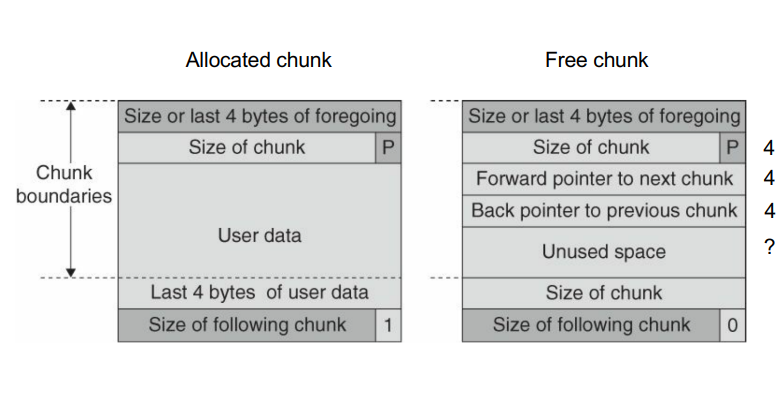
\includegraphics[width=13cm, keepaspectratio]{capitoli/secure_coding//img/cap_4/chuncks.png}
    \caption{Chunck libero e allocato.}\label{fig:chunck_lib_alloc}
\end{figure}

\subsubsection{Chunck liberi}
In dlmalloc, i blocchi liberi sono disposti in linked list
\footnote{In informatica, una lista concatenata (o linked list) è una struttura dati dinamica, tra quelle fondamentali usate nella programmazione.
    Consiste di una sequenza di nodi, ognuno contenente campi di dati arbitrari ed uno o due riferimenti ("link") che puntano al nodo successivo e/o
    precedente.}
circolari a doppio collegamento, detti anche \textbf{bin}.
Ogni linked list a doppio collegamento ha un'intestazione che contiene un puntatore in avanti e indietro rispettivamente al primo e all'ultimo blocco
nella lista. Sia il puntatore in avanti dell'ultimo chunck che quello all'indietro nel primo chunck della lista punta all'elemento testa.
Quando la lista è vuota, i puntatori della testa fanno riferimento alla testa stessa.

\subsubsection{Bin}
Ogni bin ha una \textit{head}(testa) che contiene il puntatore in avanti e indietro che puntano rispettivamente al primo e all'ultimo blocco nella lista. Sia il chunck allocato che quello libero fanno uso di un bit \verb|PREV_INUSE| (rappresentato da P \ref{fig:bin}) che indica se il chunck precedente è allocato o meno.

\begin{figure}[H]
    \centering
    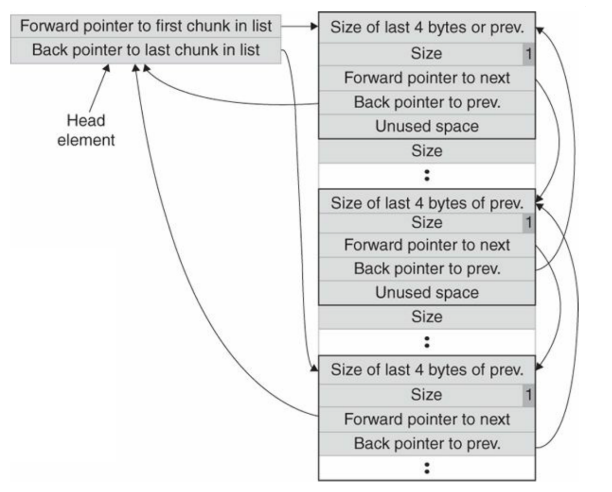
\includegraphics[width=12cm, keepaspectratio]{capitoli/secure_coding/img/cap_4/bin.png}
    \caption{Esempio di un bin.}\label{fig:bin}
\end{figure}
Sia il puntatore in avanti nell'ultimo chunck che quello indietro nel primo chunck della lista puntano alla testa. Quando la lista è vuota, la testa del puntatore si riferisce direttamente a se stessa.  Ogni
\subsubsection{UNLINK}
\verb|unlink()| è una macro usata per rimuovere un chunck dalla sua lista doppiamente linkata. Essa è usata quando la memoria è consolidata e quando un chunck è tolto della lista libera perchè è stato allocato da un utente.
\begin{verbatim}
    #define unlink(P, BK, FD) {
        FD = P -> fd;
        BK = P -> bk;
        FD -> bk = BK;
        BK -> fd = FD;
    }
\end{verbatim}

\paragraph{Funzionamento macro.}
Dalla Figura \ref{fig:ulink} si può capire bene il funzionamento della macro, essa prende in input tre puntatori
\begin{itemize}
    \item \textbf{P} puntatore al blocco da rimuovere;
    \item \textbf{BK} puntatore al blocco precedente;
    \item \textbf{FD} puntatore al blocco successivo.
\end{itemize}


\begin{figure}[H]
    \centering
    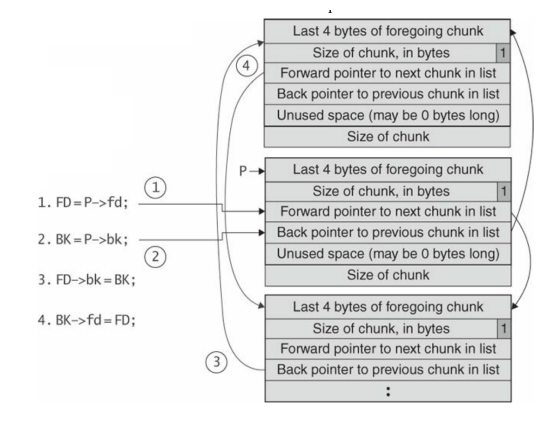
\includegraphics[width=12cm, keepaspectratio]{capitoli/secure_coding/img/cap_4/ulink.png}
    \caption{Funzionamente macro ulink.}\label{fig:ulink}
\end{figure}

In Figura \ref{fig:ulink} possiamo vedere un esempio del funzionamento della macro. Come accennato in precedenza il puntatore P si riferisce al chunck da togliere, esso contiene due puntatori uno che punta al blocco precedente e uno a quello successivo. Nel primo step della \verb|unlink()| si assegna FD in modo da farlo puntare al chunck successivo nella lista rispetto a quello indicato da P. Facciamo la stessa cosa nel secondo step solo che assegniamo a BK il puntatore al chunck precedente. Nel terzo step, il puntatore in avanti (FD)  sostituisce il puntatore all'indietro del blocco successivo nella lista con il puntatore al blocco che precede quello che è stato scollegato. Nell'ultimo step il puntatore all'indietro (BK) sostituisce il puntatore in avanti del precedente chunck nella lista con il puntatore al blocco successivo.

\subsection{Tecnica unlink}
La tecnica unlink è stata introdotta la prima volta da Solar Designer e usata con successo contro alcune versioni dei browser di Netscape, traceroute e slocate che utilizzavano dlmalloc. Questa tecnica è usata per fare un buffer overflow in modo da manipolare i tag di confine su un chunck di memoria per ingannare la macro \verb|unlink()| facendole scrivere 4 byte di dati in una zona arbitraria.

\begin{figure}[H]
    \centering
    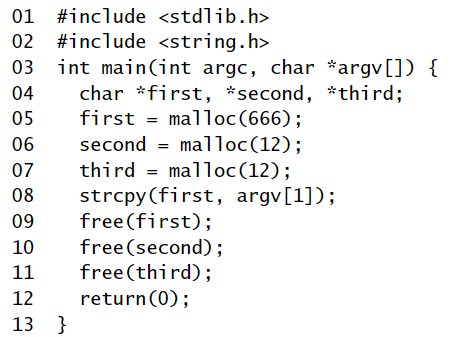
\includegraphics[width=10cm, keepaspectratio]{capitoli/secure_coding/img/cap_4/unlink_buff_over.png}
    \caption{Esempio di codice vulnerabile a tecnica unlink.}\label{fig:ulink_buff_over}
\end{figure}

Il programma vulnerabile alloca 3 chunck di memoria (riga 5-7). Il programma accetta una singola stringa come argomento che è copiata all'interno della malloc \textit{first} (linea 8). Questa operazione strcpy() illimitata è soggetta a un buffer overflow. Il tag di confine può essere sovrascritto da un argomento stringa che supera la lunghezza di first perché il tag di confine per il secondo si trova direttamente dopo il primo buffer. Il problema di questo programma accade alla seconda free (linea 10). Vediamo come è strutturato l'heap prima di fare la seconda free.

\begin{figure}[H]
    \centering
    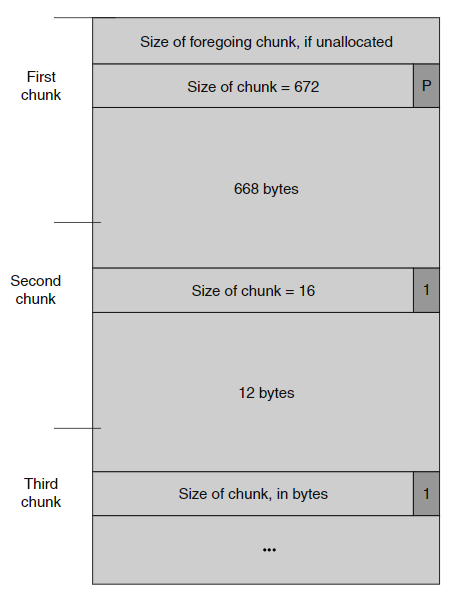
\includegraphics[width=10cm, keepaspectratio]{capitoli/secure_coding/img/cap_4/heap_prima_free.png}
    \caption{Contenuto dell'heap alla prima chiamata di free().}\label{fig:heap_prima_free}
\end{figure}
Se il secondo blocco non è allocato, l'operazione \verb|free()| prova a consolidarlo con il primo blocco. Per determinare se il secondo chunck è allocato o meno bisogna guardare il \verb|PREV_INUSE| bit del terzo blocco. La locazione di ogni blocco è determinata aggiungendo la grandezza del blocco all'indirizzo iniziale. Durante le operazioni normali, il bit P del terzo chunck è settato perchè il secondo chunck è allocato come si vede in Figura \ref{fig:heap_prima_free}.
Poiché il buffer vulnerabile è allocato nell'heap e non nello stack, l'attaccante non può solamente sovrascrivere l'indirizzo di ritorno per sfruttare la vulnerabilità ed eseguire codice malevolo. L'attaccante può sovrascrivere i boundary tag associati con il secondo chunck della memoria, perchè questo tag di confine è collocato immediatamente dopo la fine del primo blocco. La grandezza del primo chunck (672 byte) è il risultato della grandezza richiesta di 666 byte, più 4 byte per la grandezza, arrotondato al multiple più vicino a 8 poichè tutti chunck devono essere divisibili per 8 byte.
\begin{figure}[H]
    \centering
    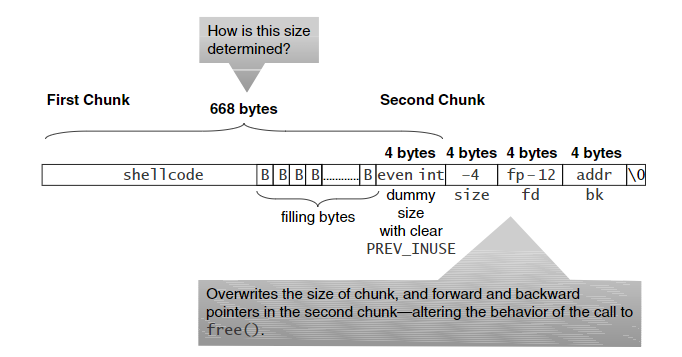
\includegraphics[width=13cm, keepaspectratio]{capitoli/secure_coding/img/cap_4/funzionamento_unlink.png}
    \caption{Funzionamento tecnica unlink.}\label{fig:funzionamento_unlink}
\end{figure}
Come si vede in Figura \ref{fig:funzionamento_unlink} un argomento malevolo può essere usato per sovrascrivere i tag del secondo chunck. Questo argomento sovrascrive il campo della dimensione del precedente blocco, grandezza del chunck, e i puntatori in avanti e indietro del secondo chunck, alterando così il comportamento della free(). In particolare il campo per la dimensione è modificato inserendo come valore -4 byte, in questo modo quando la free() prova a determinare la locazione del terzo chunck aggiungendo la grandezza appena modificata all'indirizzo iniziale del secondo chunck invece di aggiungere sottrae 4 byte. Così la dlmalloc pensa che l'inizio del successivo chunck è 4 byte prima dell'inizio del secondo chunck. L'argomento malevolo garantisce che la collocazione dove la dlmalloc trova il bit P è libera, ingannando la dlmalloc facendole credere che il secondo chunck non è allocato così l'operazione di free() invoca la unlink macro per consolidare i due blocchi liberi consecutivi. Come si vede in Figura \ref{fig:funzionamento_unlink} viene inserito al posto della grandezza effettiva del chunck un numero pari finto, deve essere pari poiché l'ultimo bit deve essere 0.  In fd inseriamo \verb|fp-12| che è l’indirizzo dove voglio compiere l’attacco. In bk c’è il dato che vogliamo scrivere all’indirizzo fd.
Per come è scritta la unlink, è lei stessa che fa questa cosa quando viene chiamata la seconda free.
Noi scriviamo solo il payload, poi il lavoro lo fanno free e di conseguenza unlink. L'obiettivo è scrivere l'indirizzo addr in fp.

